\subsection{Inputs}

The performance of the CNN tagger strongly depends on the choice of physics objects used to build the input images.
Each input type is affected by experimental effects in different ways. 
Tracks only account for the charged particles in the jet; 
calorimeter towers include both charged and neutral component of the shower, but do not attempt to resolve individual particles. 
Calorimeter clusters aim at retaining the full granularity of the calorimeters while applying a zero suppression. 
They often merge close by particles and have a worse energy resolution than the track momentum resolution at low 
and moderate particle $p_\text{T}$.
In addition, both calorimeter towers and clusters are more strongly affected by pile-up contributions.
Figure~\ref{fig:cnn-input} shows that the best discriminating performance is achieved by combining tower or topocluster images and track images as input for the CNN tagger.
The two types of image are stacked so that the input to the CNN is a multi-dimensional array of size $16\times 16\times 2$.
In the lower $p_\text{T}$ range shown in Fig.~\ref{fig:cnn-input}, this combination actually saturates the achievable performance at low $p_\text{T}$ bound set by using truth particles.  
There is a small gap in the higher $p_\text{T}$ bin, suggesting further experimental improvements may help improve performance. 

\begin{figure}[htpb]
\begin{center}
\subfloat[][]{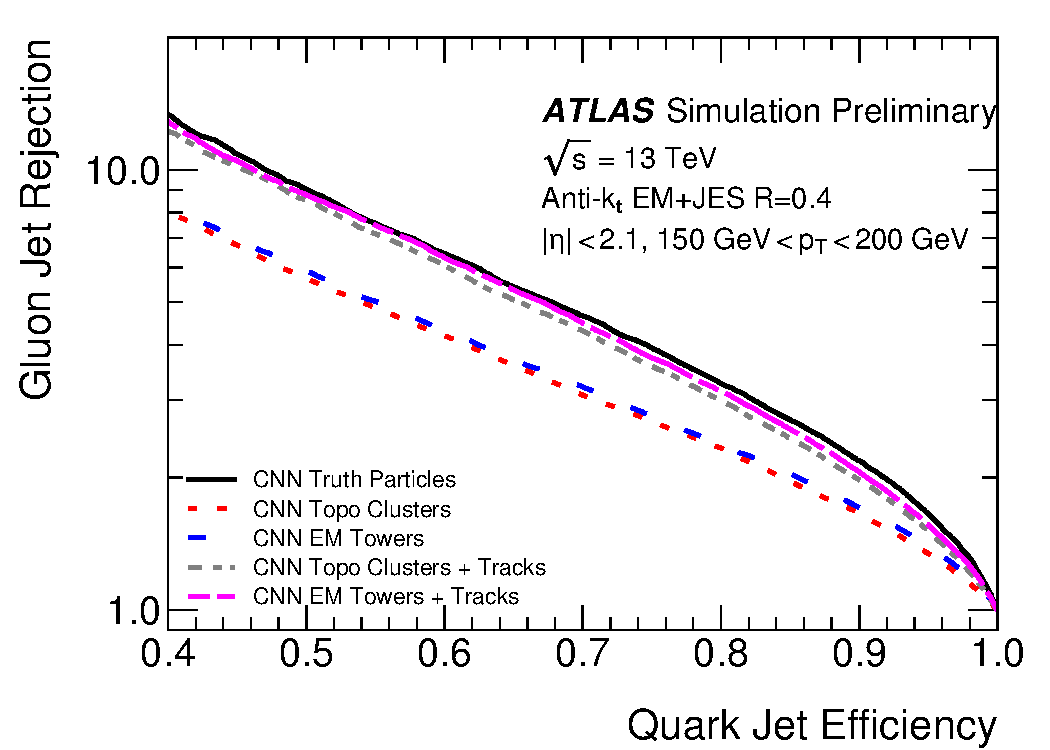
\includegraphics[width=0.5\textwidth]{figures/CNN/ROC_pt150_200_input.pdf}\label{lowpt}}
\subfloat[][]{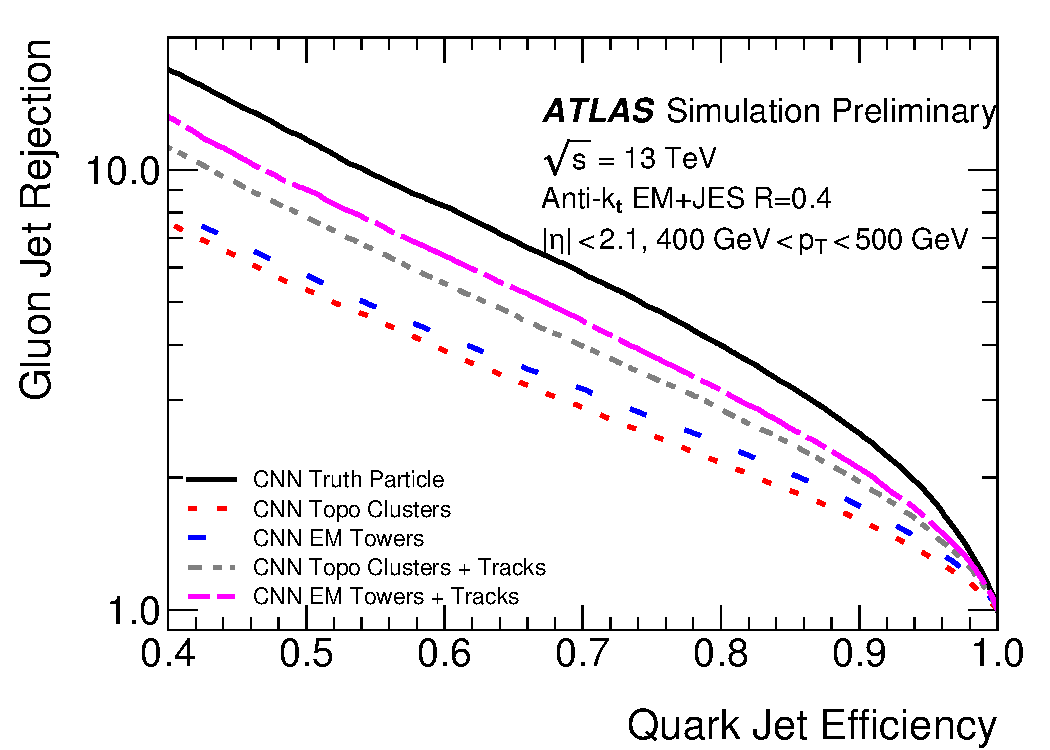
\includegraphics[width=0.5\textwidth]{figures/CNN/ROC_pt400_500_input.pdf}\label{highpt}}
\caption{Gluon jet rejection as a function of the quark jet efficiency using the CNN tagger with different inputs
for jets with \protect\subref{lowpt} $150<\pt<200~\GeV$ and \protect\subref{highpt} $400<\pt<500~\GeV$.}
\label{fig:cnn-input}
\end{center}
\end{figure}

The difference between the full truth-particle line and the calorimeter + reconstructed tracks lines in Figure~\ref{fig:cnn-input} 
depends on many details of the detector response, angular resolution, reconstruction efficiency, etc.  
However, it is possible to isolate one component of the difference by focusing only on the charged-particles.  Figure~\ref{fig:cnn-tracktruth}(a) shows the performance of a track-only-image at both particle-level and detector-level.  As might be expected, due to the precise measurement of charged-particle trajectories, there is little difference between the particle- and detector-levels.  Degradation due to efficiency and resolution effects are only expected at much lower and higher transverse momenta.

\begin{figure}[htpb]
\begin{center}
\subfloat[][]{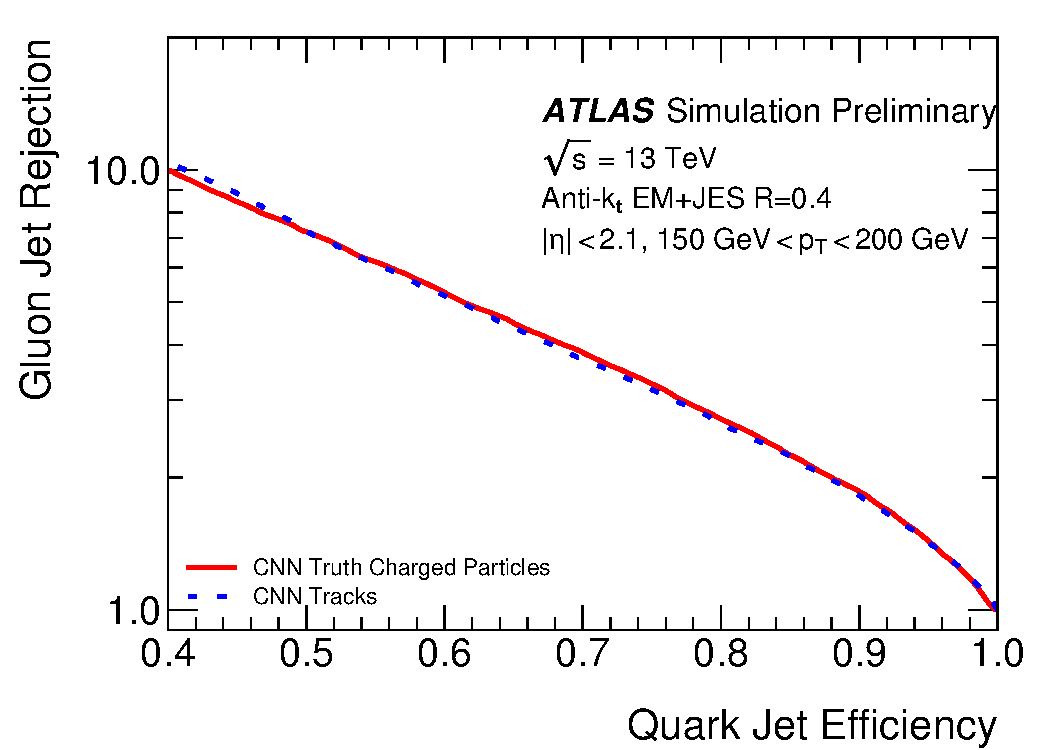
\includegraphics[width=0.5\textwidth]{figures/CNN/ROC_pt150_200_track.pdf}\label{tracktruth}}
\subfloat[][]{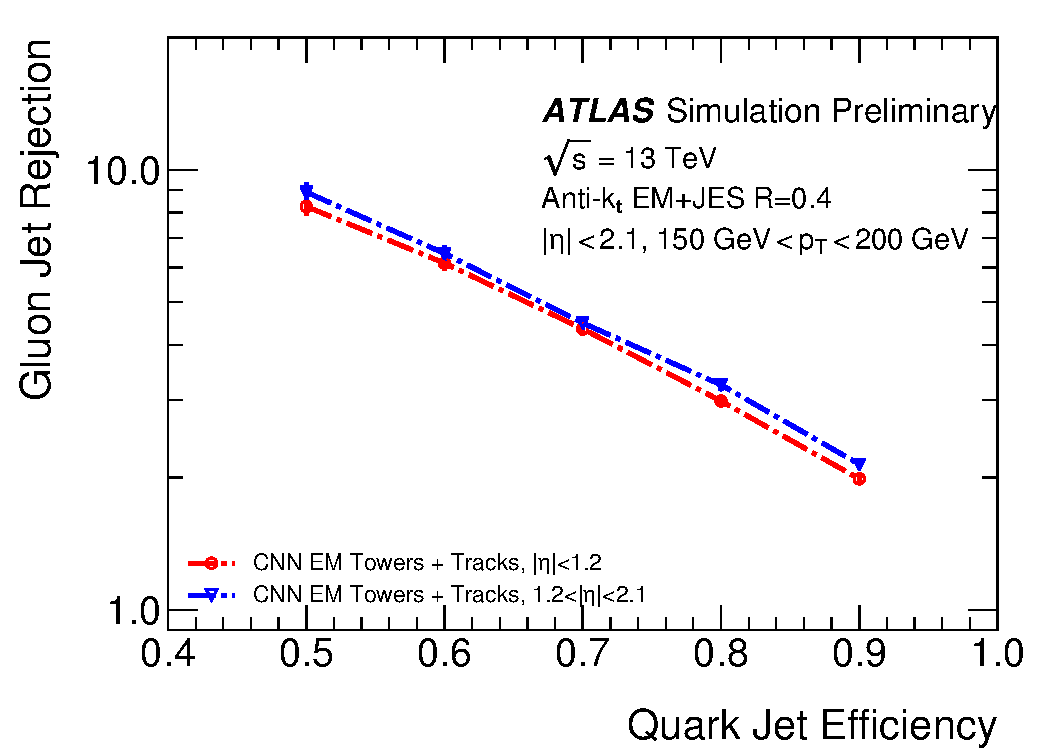
\includegraphics[width=0.5\textwidth]{figures/CNN/ROC_pt150_200_eta.pdf}  \label{kinematics}}
\caption{Gluon jet rejection as a function of the quark jet efficiency using the CNN tagger for jets with $150<\pt<200~\GeV$.
\protect\subref{tracktruth} Comparison between using track images and truth charge particle images as input.
\protect\subref{kinematics} Comparison between different $|\eta|$ ranges. The full $|\eta|$ range ($|\eta|<2.1$) is used for training.}
\label{fig:cnn-tracktruth}
\end{center}
\end{figure}

\subsection{Pile-ups}

The impact of pileup effects on the performance of the CNN tagger is evaluated 
by considering events with a different number of reconstructed primary vertices ($N_\text{PV}$).
The test sample is divided into three bins: $N_\text{PV}<13$, $13<N_\text{PV}<20$ and $N_\text{PV}>20$.  
The distributions of the pixel intensities do vary with pileup, 
but the performance of the CNN tagger is found to be robust. 
This is demonstrated by Figure~\ref{fig:cnn-pileup}. 
% shows that the efficiencies for a specific working point vary with the pileup conditions (by a similar amount as jet width), but the overall discriminating performance is not significantly degraded (ROC curve is largely invariant).

\begin{figure}[htpb]
\begin{center}
\includegraphics[width=0.5\textwidth]{figures/CNN/ROC_pt150_200_NPV.pdf}
%\subfloat[][]{\includegraphics[width=0.5\textwidth]{figures/roc/ROC_pt150_200_NPV.pdf}\label{roc}}
%\subfloat[][]{\includegraphics[width=0.5\textwidth]{figures/roc/NPVEff.pdf}\label{eff}}
\caption{Gluon jet rejection as a function of the quark jet efficiency %\protect\subref{roc} 
evaluated at different pileup conditions, 
quantified by the number of reconstructed primary vertices ($N_\text{PV}$).}
%\protect\subref{eff} 
%Quark and gluon jet efficiency as a function of NPV for the CNN tagger.
%Jets are selected by requiring a minimum value of the CNN tagger, 
%where the threshold is chosen to give an overall 60\% quark jet efficiency.
%The efficiencies for jet width are shown for reference.}
\label{fig:cnn-pileup}
\end{center}
\end{figure}

Calorimeter-based discrimination is not only effected by in-time pileup (quantified by $N_\text{PV}$) but also by out-of-time pileup. 
Figure~\ref{fig:cnn-pileup2} compares the tagger performance in two different regimes of the average number of collisions per bunch crossing ($\mu$) regimes corresponding to the out-of-time pileup representative of LHC Run 2 conditions.

\begin{figure}[htpb]
\begin{center}
\subfloat[][]{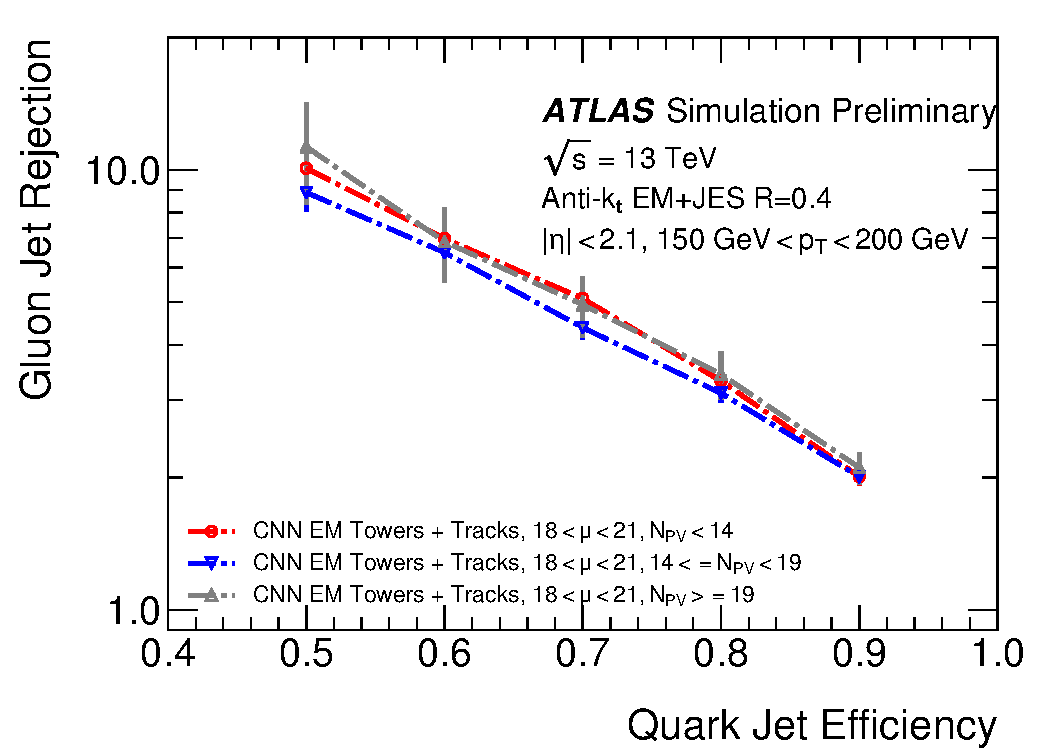
\includegraphics[width=0.5\textwidth]{figures/CNN/ROC_pt150_200_mu18_21.pdf}\label{roc1}}
\subfloat[][]{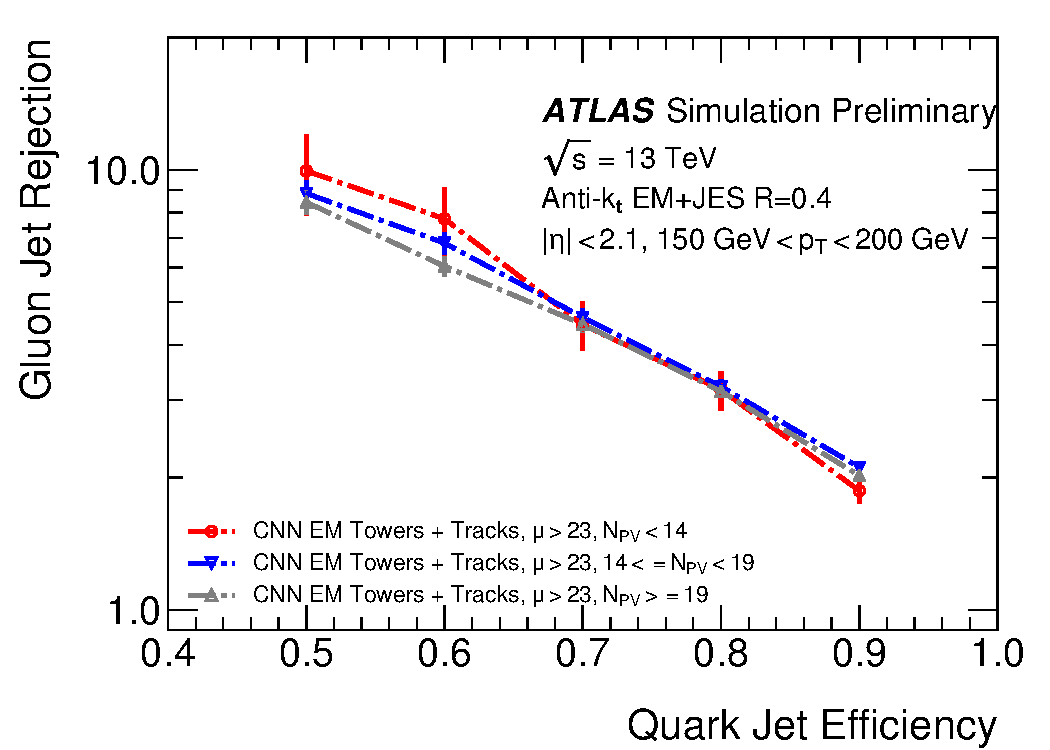
\includegraphics[width=0.5\textwidth]{figures/CNN/ROC_pt150_200_mu23.pdf}\label{roc2}}
\caption{Gluon jet rejection as a function of the quark jet efficiency 
evaluated at different levels of $N_\text{PV}$ for \protect\subref{roc1} $18<\mu<23$ and \protect\subref{roc2}  $\mu > 23$.
The two $\mu$ bins where chosen to have roughly the same number of events.}
\label{fig:cnn-pileup2}
\end{center}
\end{figure}


\subsection{Modeling}

Quark versus gluon tagging is sensitive to the detailed modeling of perturbative and non-perturbative effects involved with fragmentation.  
We compare images and image classification performance with two very different fragmentation models.  
Figure~\ref{fig:cnn-avg:pythiasherpa} shows the average image (differences) between quark and gluon jets simulated with 
\textsc{Pythia} 8 and with \textsc{Herwig++}.  
The radiation pattern inside gluon jets is similar between the two models, whereas there are larger differences for quark jets.  
In particular, quark and gluon jets are more different according to \textsc{Pythia} 8 relative to \textsc{Herwig++}.  
This is observed with the CNN in Fig.~\ref{fig:cnn-pythiasherpa}.  
As gluon jets in \textsc{Herwig++} are more similar to quark jets than in \textsc{Pythia} 8, 
any observable (including the CNN tagger output) tends to have less discrimination power when tested in \textsc{Herwig++}.
The training sample determines the nature of the observable the CNN tagger learns. 
By comparing the CNN tagger trained on \textsc{Pythia} 8 events with the one trained on \textsc{Herwig++} events
using the same test sample (\textsc{Pythia} 8),
we see a smaller discrepancy, indicating that the learned feature is not strongly sensitive 
to the difference between \textsc{Pythia} 8 and \textsc{Herwig++}.
\textsc{Pythia} 8 and \textsc{Sherpa} produce relatively similar images and so unsurprisingly, 
the CNN performance is similar when trained/tested on either of these generators.  
As also noted by Ref.~\cite{Barnard:2016qma}, when generators produce different images, 
the CNN returns a different performance when training and testing with images from various simulators.  
However, if the same network is used for testing and only the training sample is varied, 
the gap in performance is mostly removed (see also~\cite{Komiske:2016rsd}).  
One explanation is that the network is learning robust features for quark versus gluon tagging, 
but the degree to which the features are expressed in the radiation patterns varies between generators.

\begin{figure}[htpb]
\begin{center}
  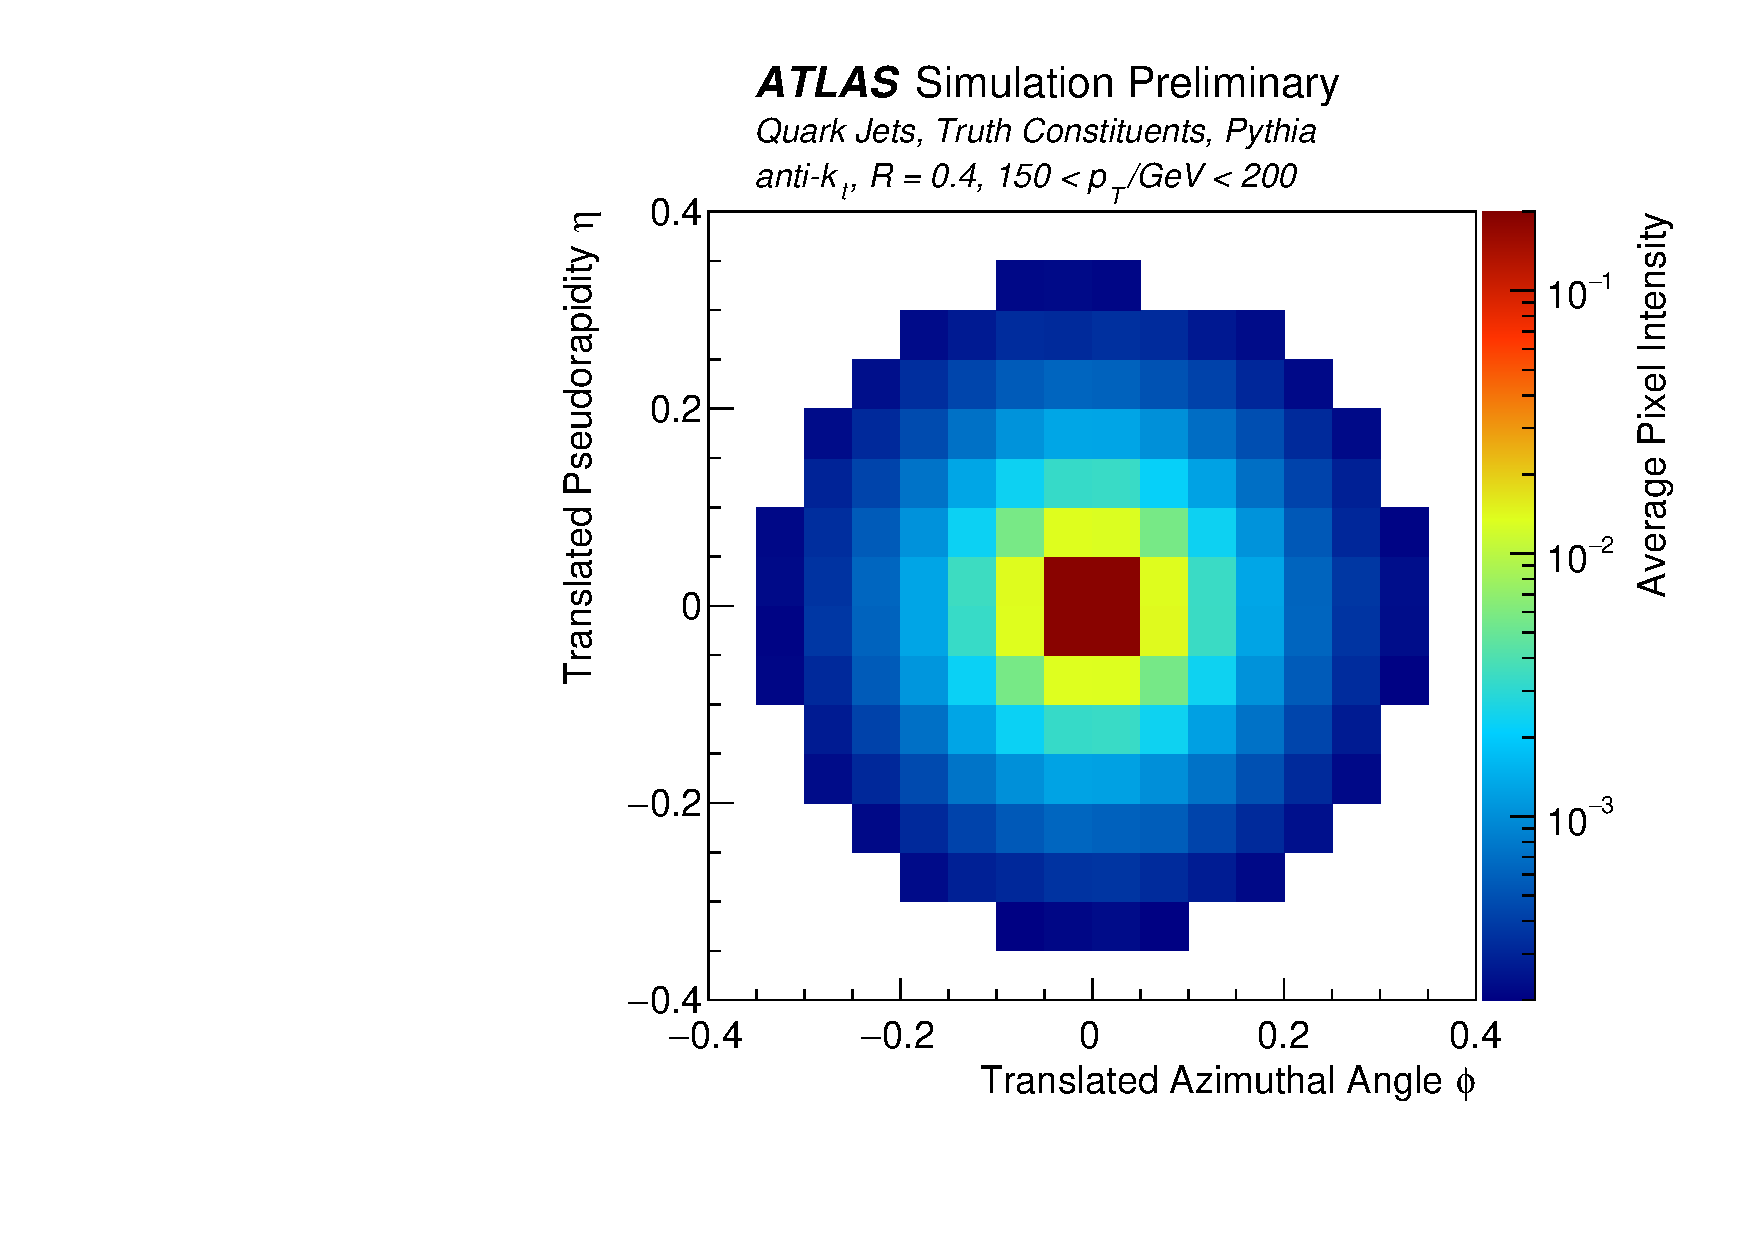
\includegraphics[width=0.31\textwidth]{figures/CNN/quark_truth_pythia.pdf}
  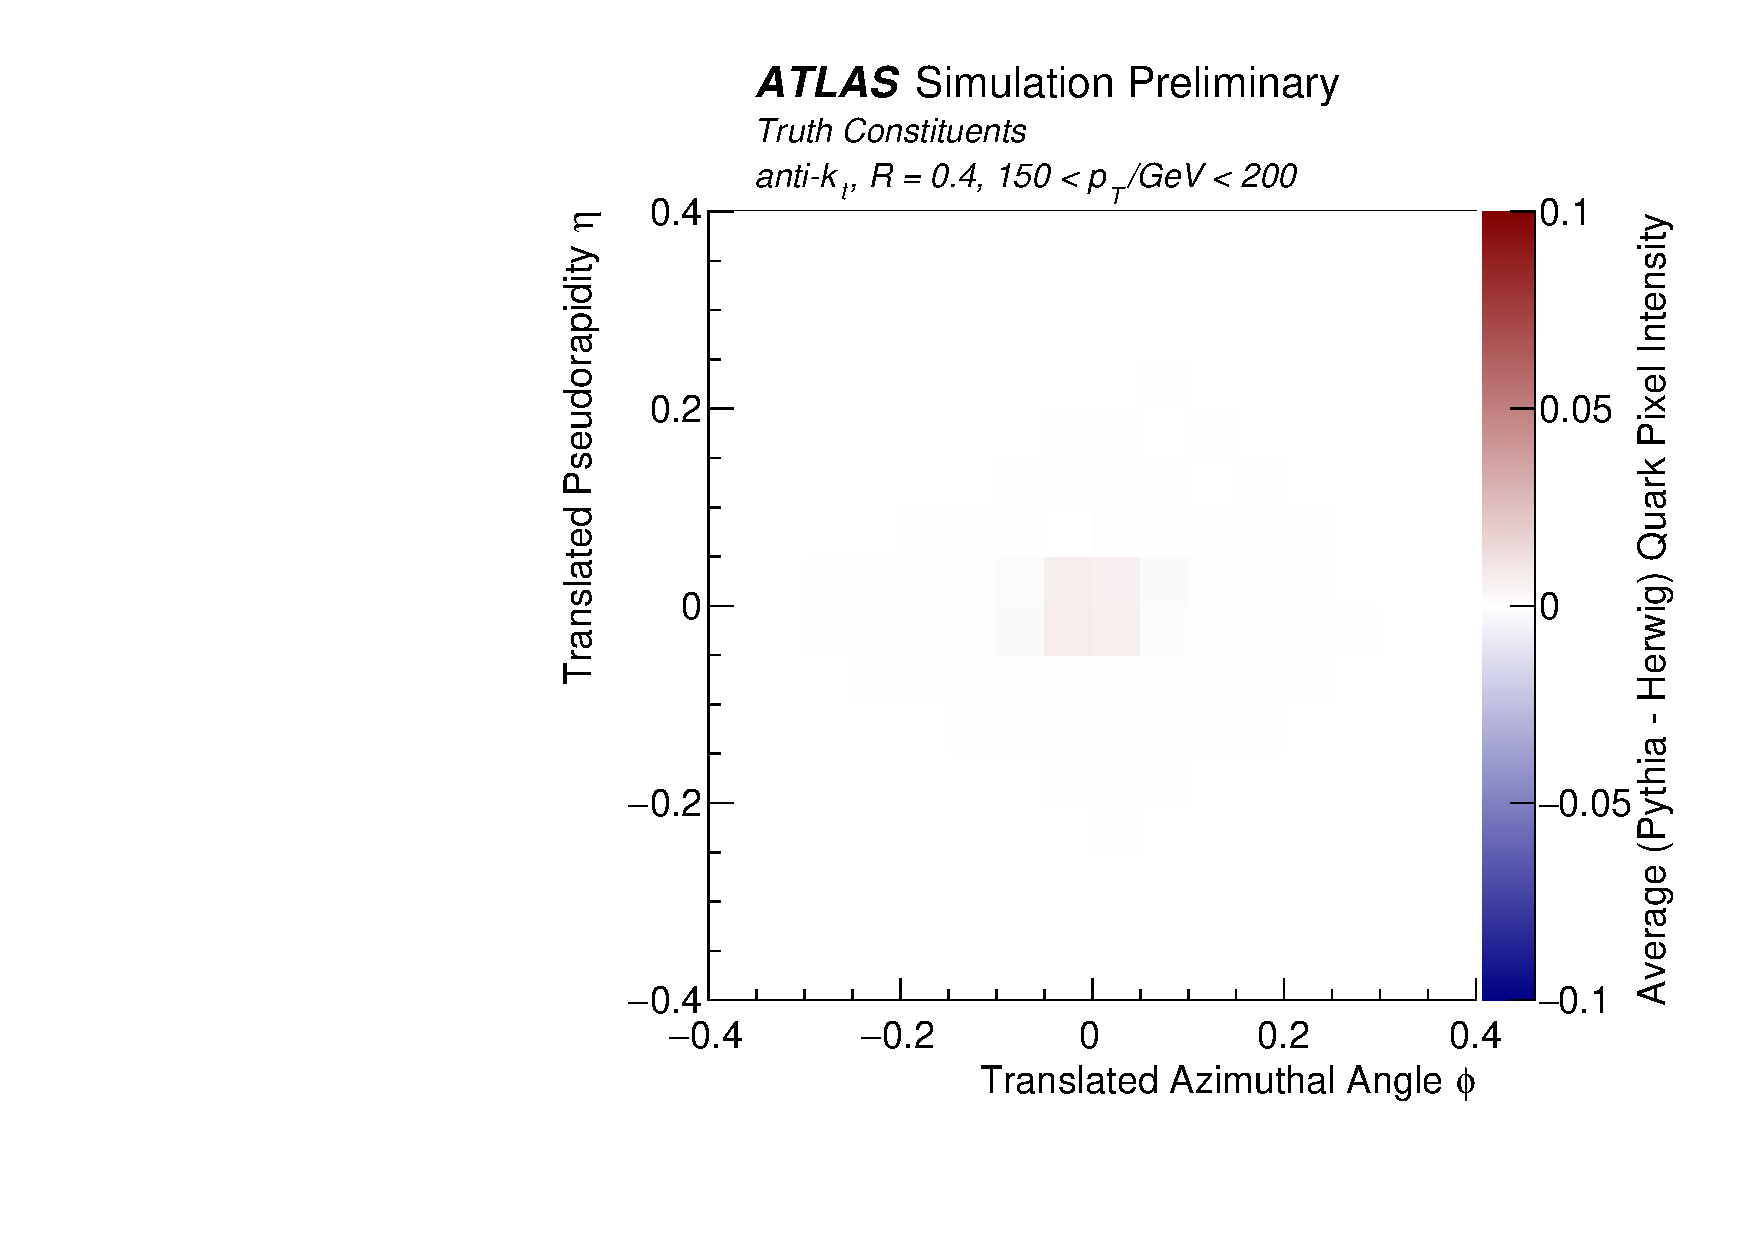
\includegraphics[width=0.31\textwidth]{figures/CNN/diff_truthq_pythiaherwig.pdf}
  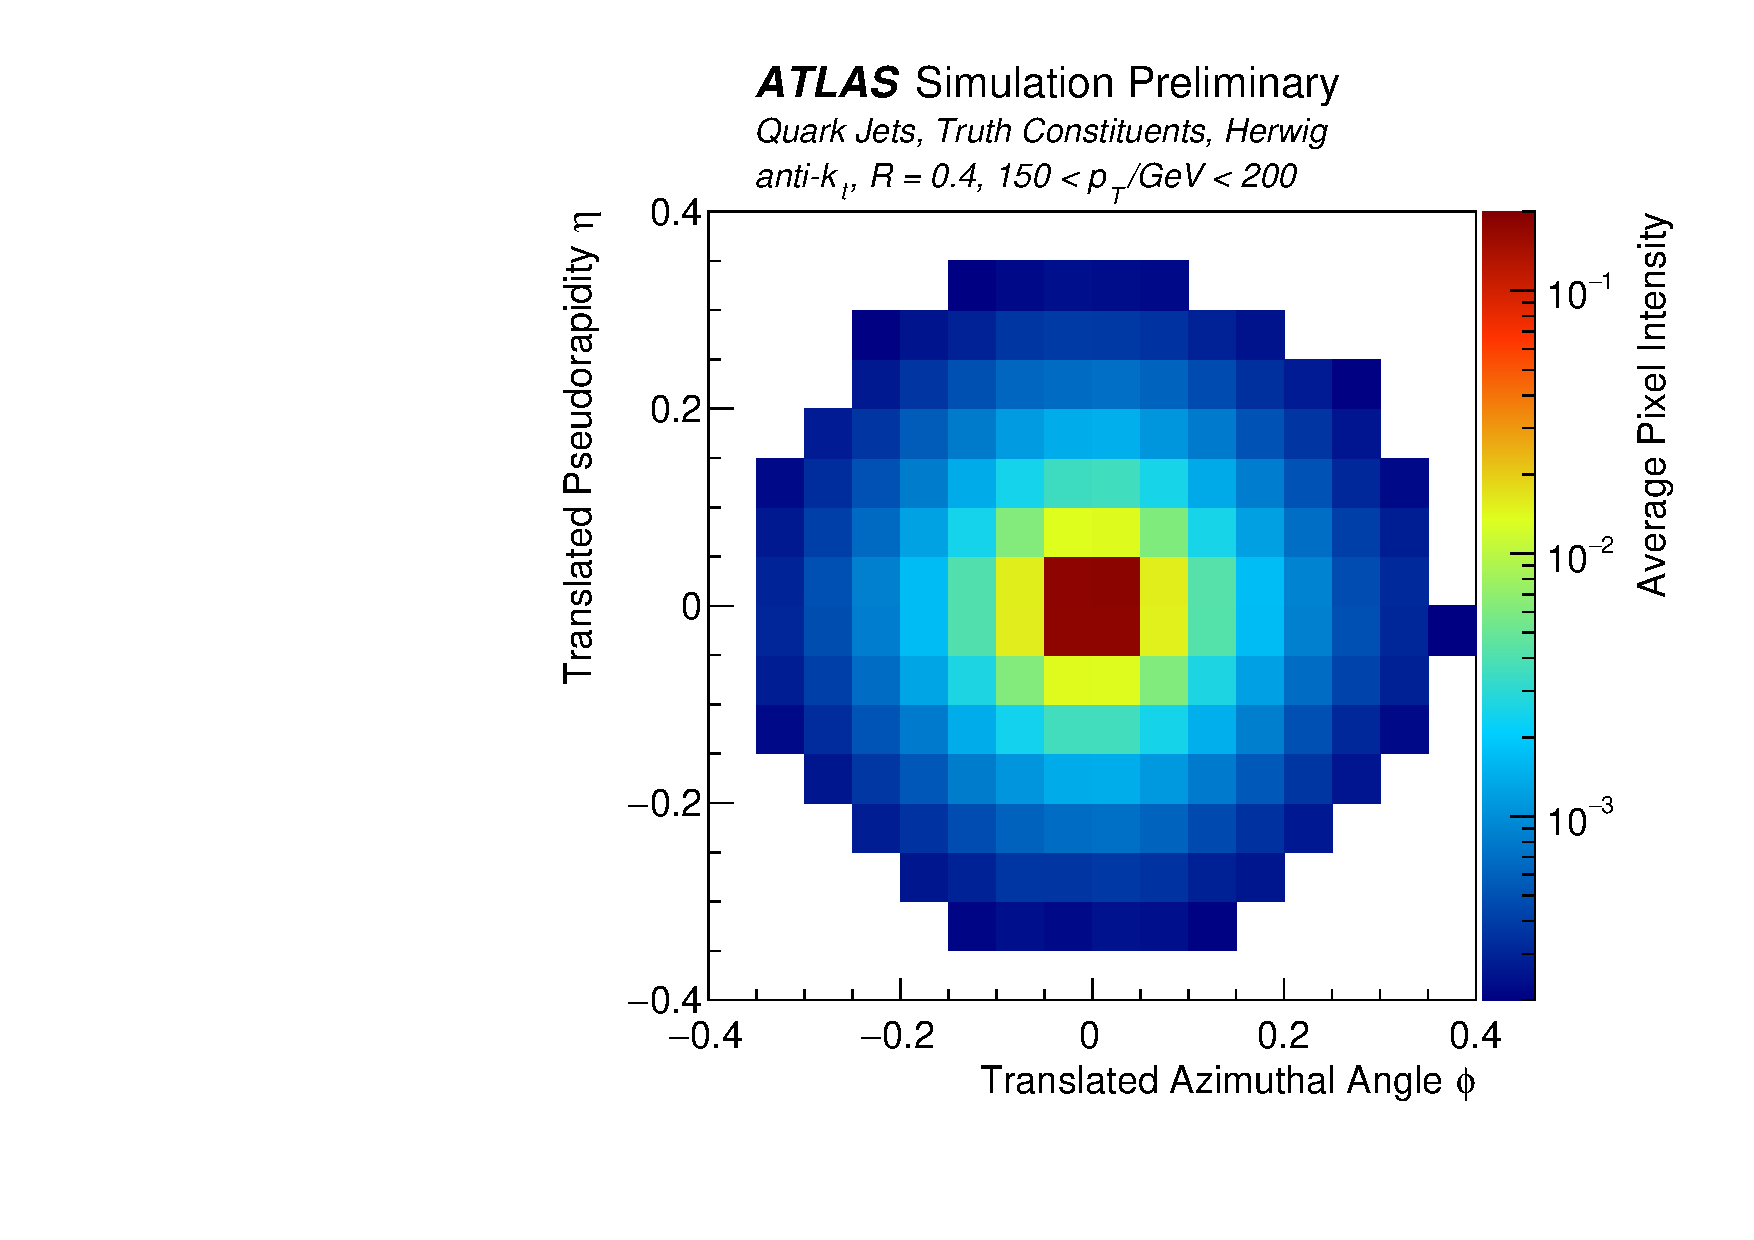
\includegraphics[width=0.31\textwidth]{figures/CNN/quark_truth_herwig.pdf}\\
  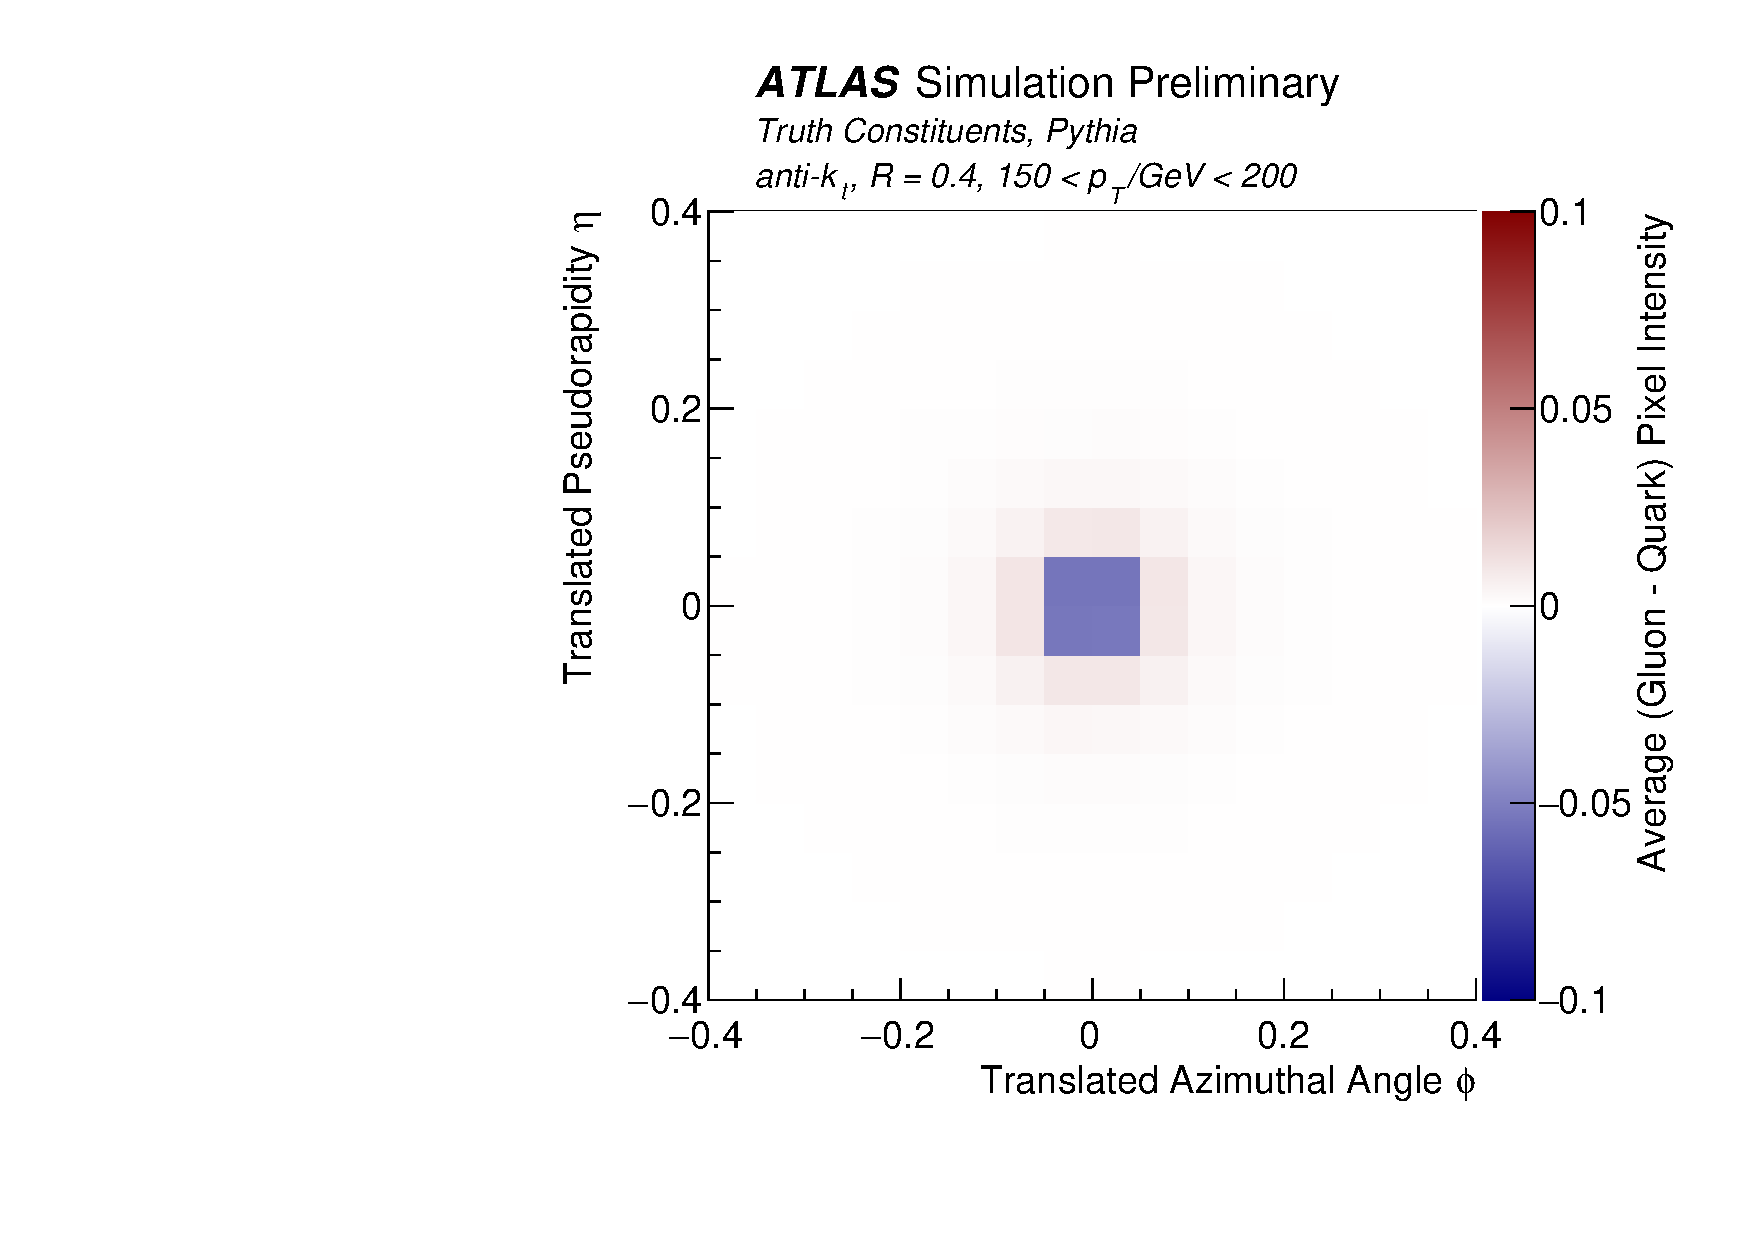
\includegraphics[width=0.31\textwidth]{figures/CNN/diff_truth_pythia.pdf}\hspace{54mm}
  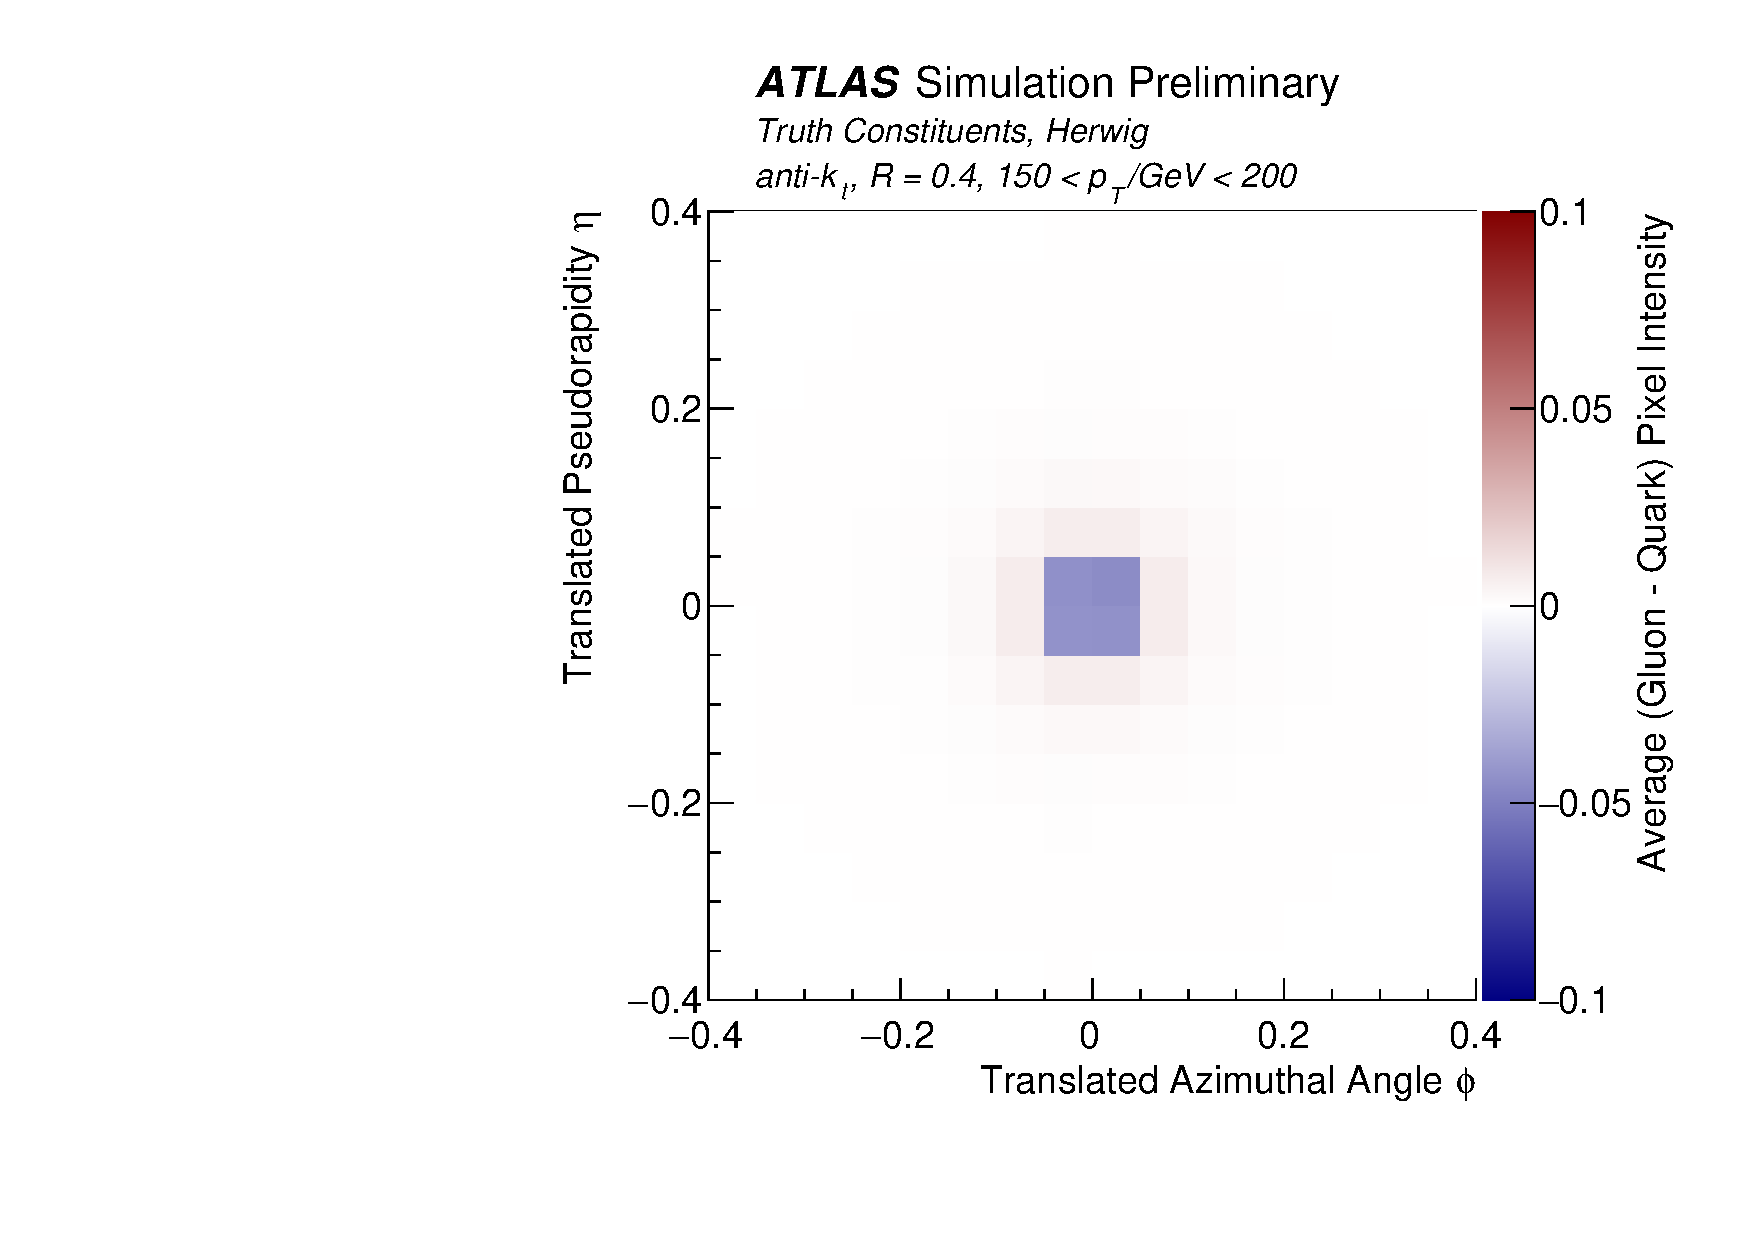
\includegraphics[width=0.31\textwidth]{figures/CNN/diff_truth_herwig.pdf}\\
  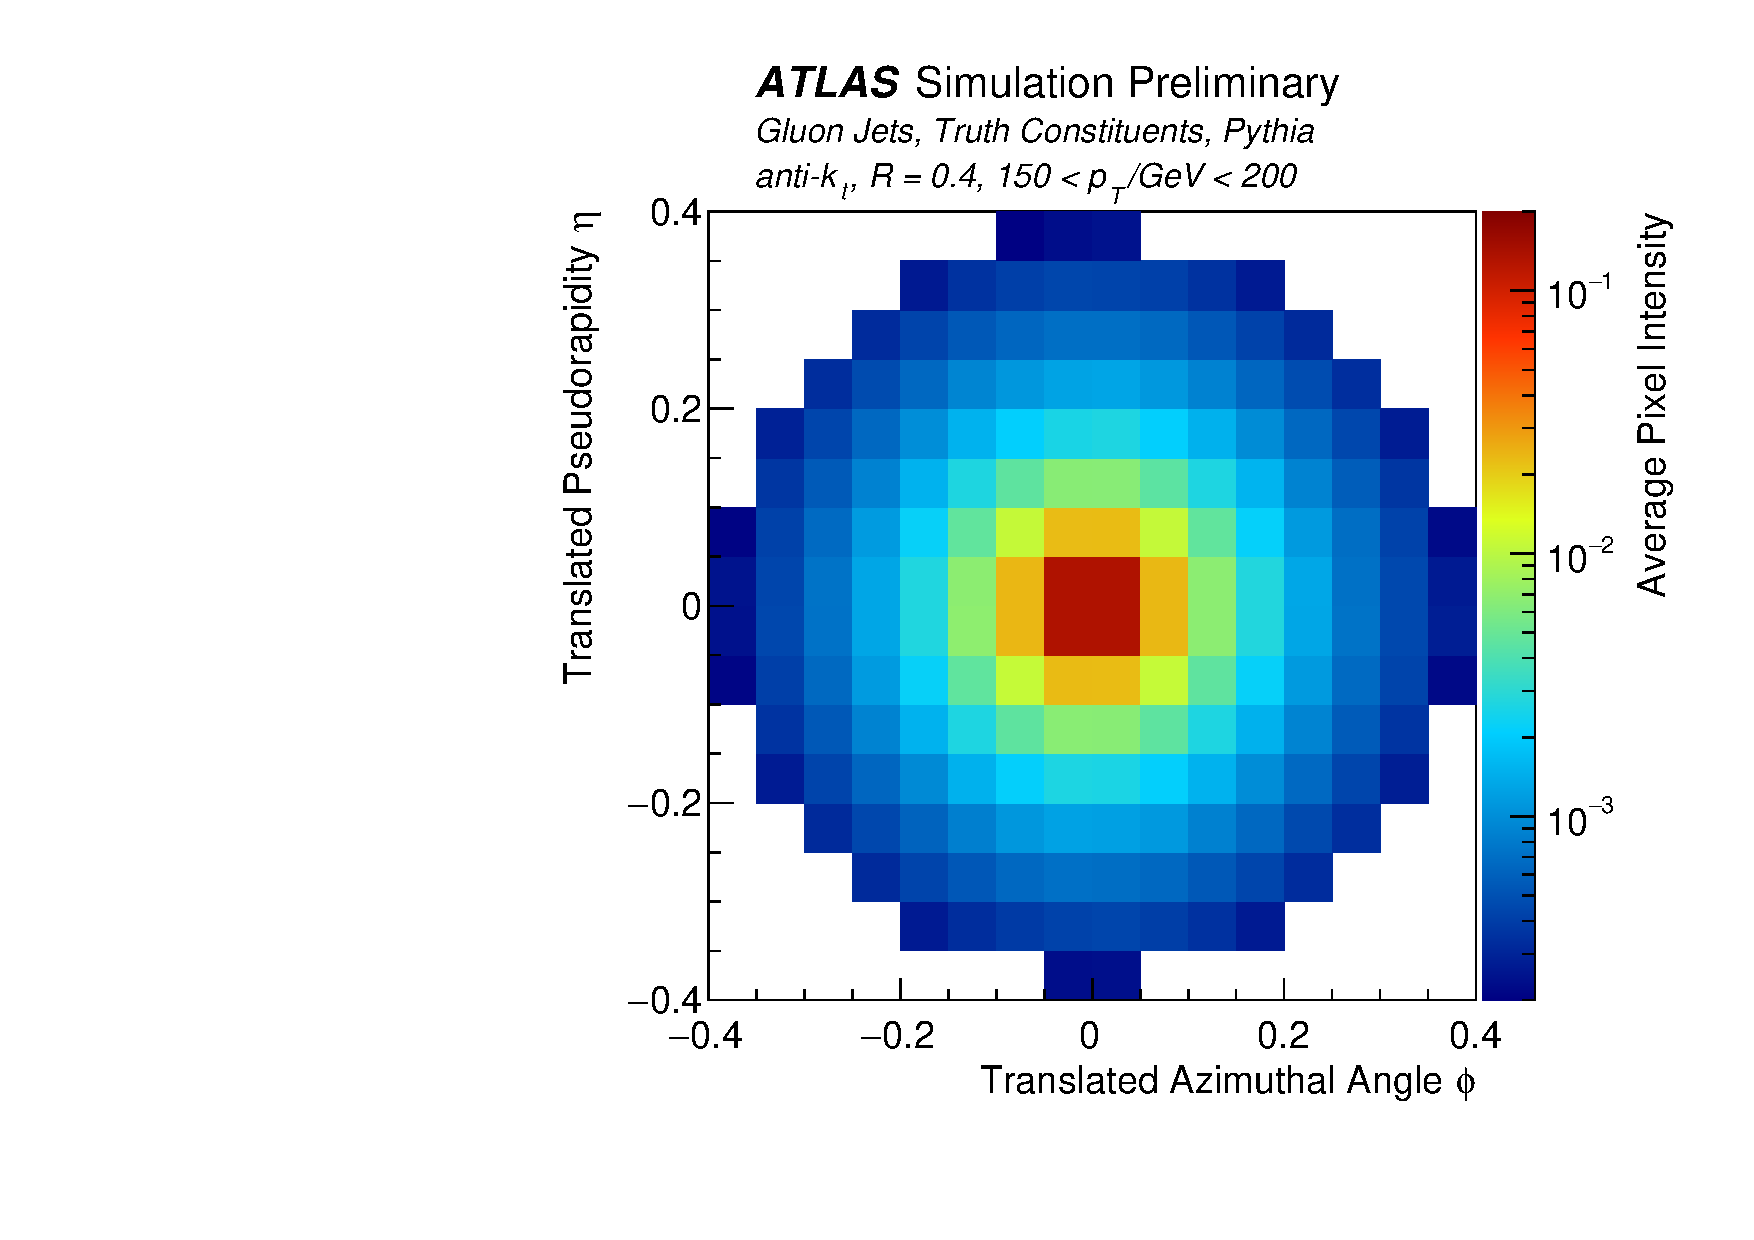
\includegraphics[width=0.31\textwidth]{figures/CNN/gluon_truth_pythia.pdf}
  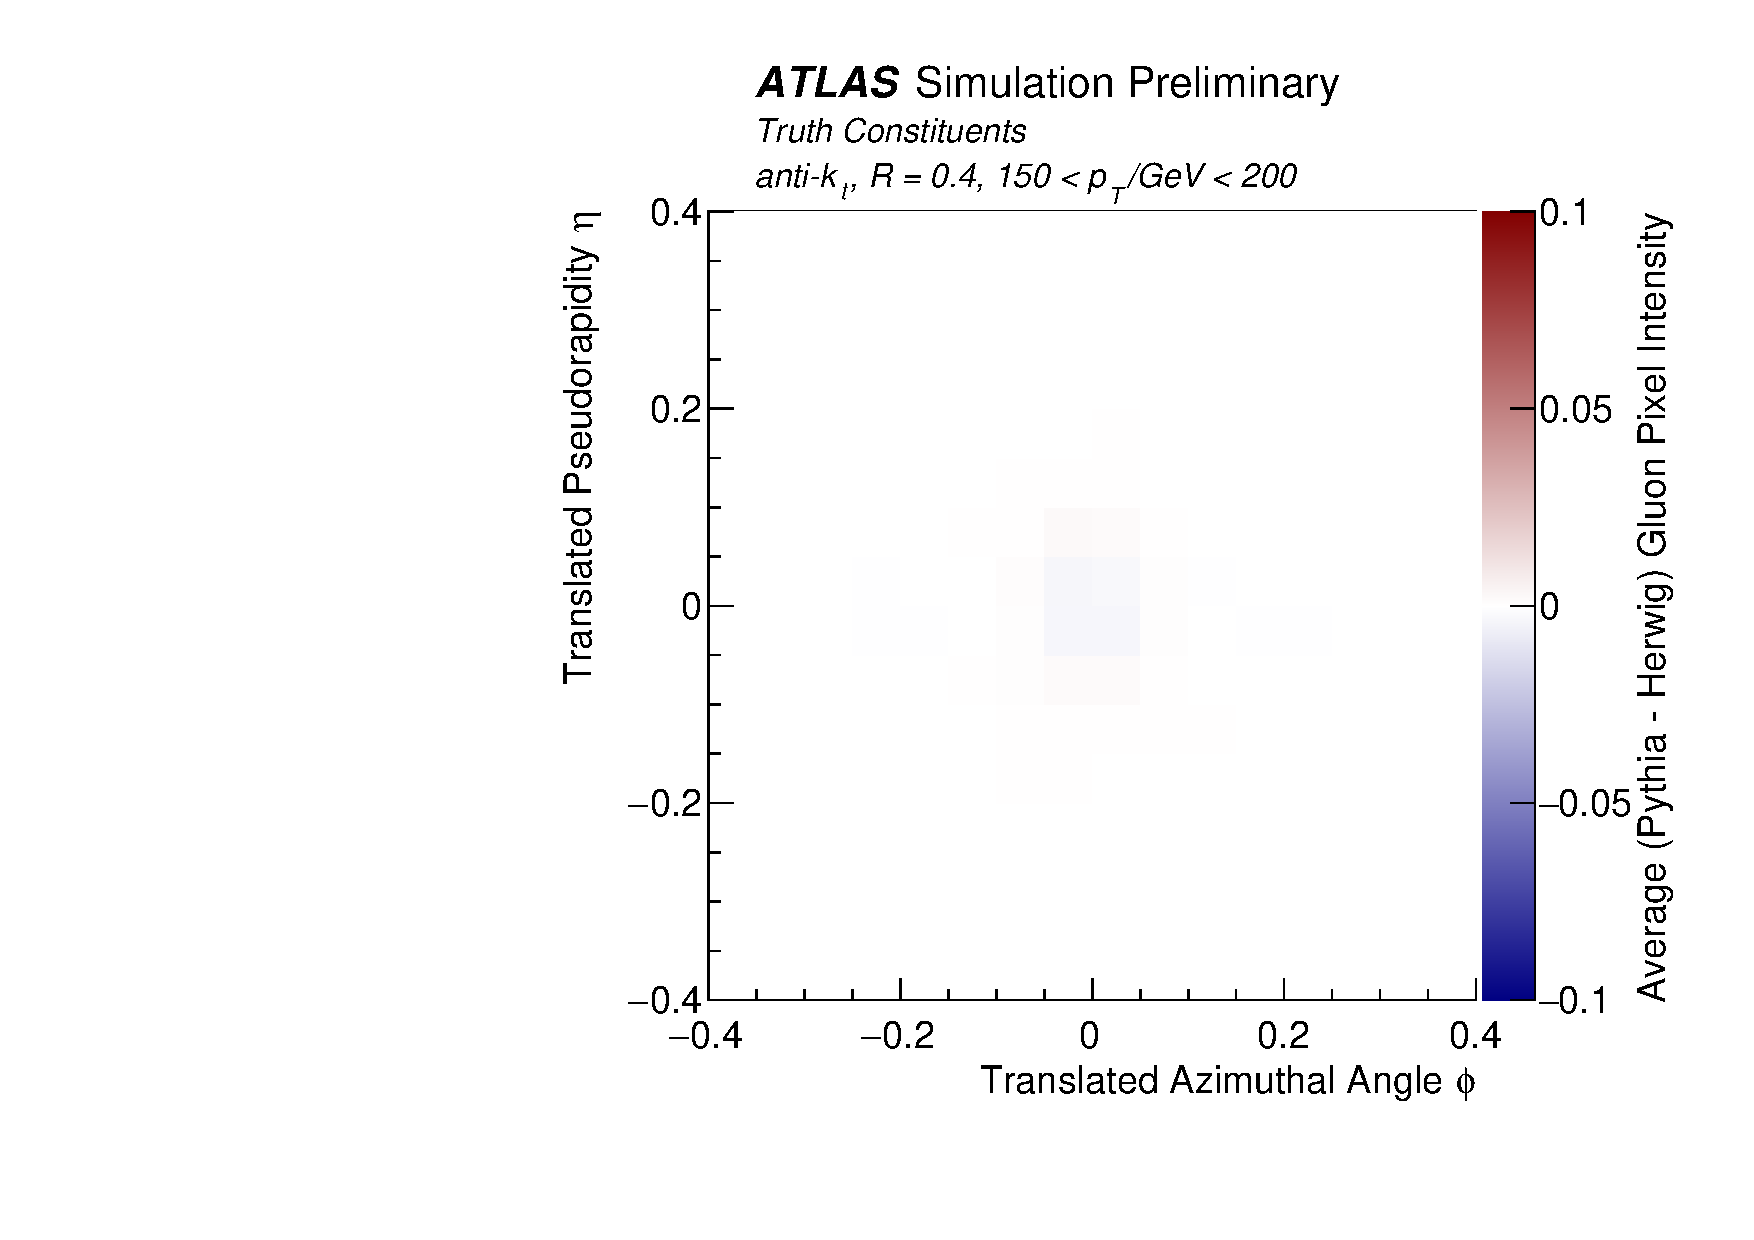
\includegraphics[width=0.31\textwidth]{figures/CNN/diff_truthg_pythiaherwig.pdf}
  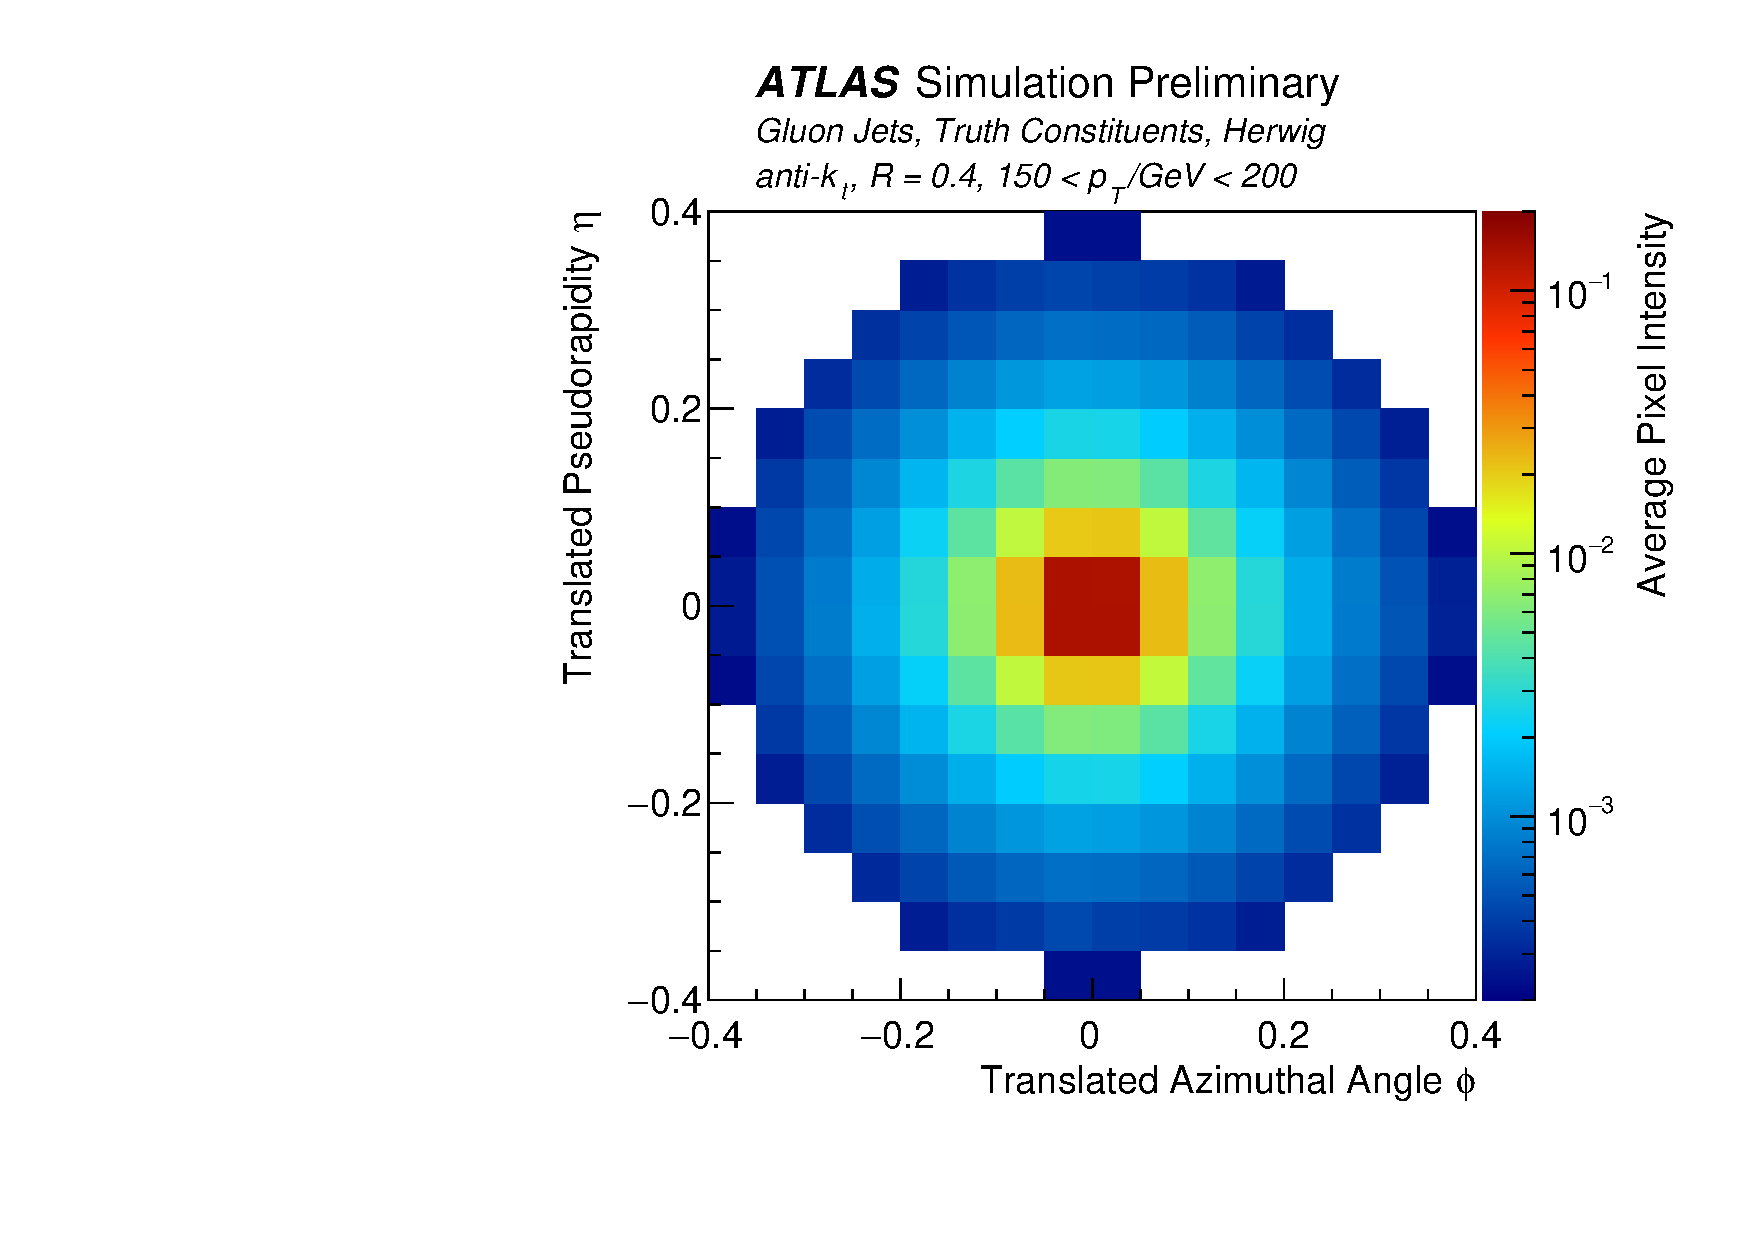
\includegraphics[width=0.31\textwidth]{figures/CNN/gluon_truth_herwig.pdf}
\caption{
The four corners show the average quark (top) and gluon (bottom) jet images, for jets generated with \textsc{Pythia} (left) and
and \textsc{Herwig} (right); the four plots on the edges show the difference between the adjacent plots,
for example the top plot shows the difference between the average quark jet in \textsc{Pythia} and
and \textsc{Herwig}.}
\label{fig:cnn-avg:CNN}
\end{center}
\end{figure}


\begin{figure}[htpb]
\begin{center}
\subfloat[][]{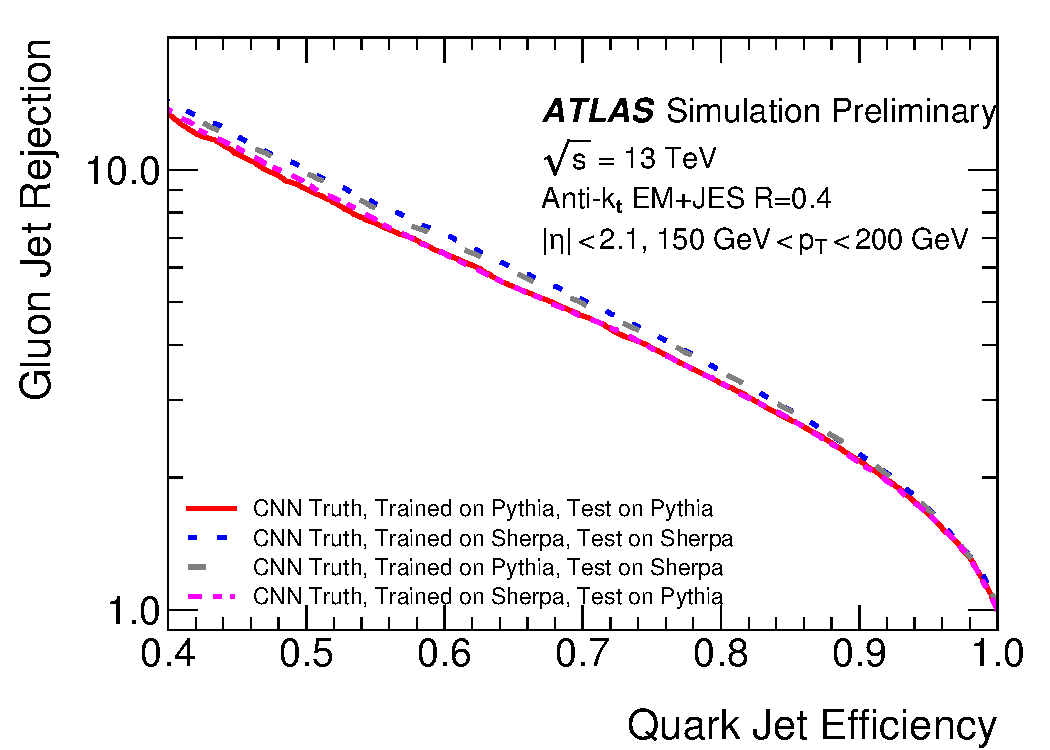
\includegraphics[width=0.5\textwidth]{figures/CNN/ROC_pt150_200_gen_pythia_sherpa.pdf}\label{CNN}} 
\subfloat[][]{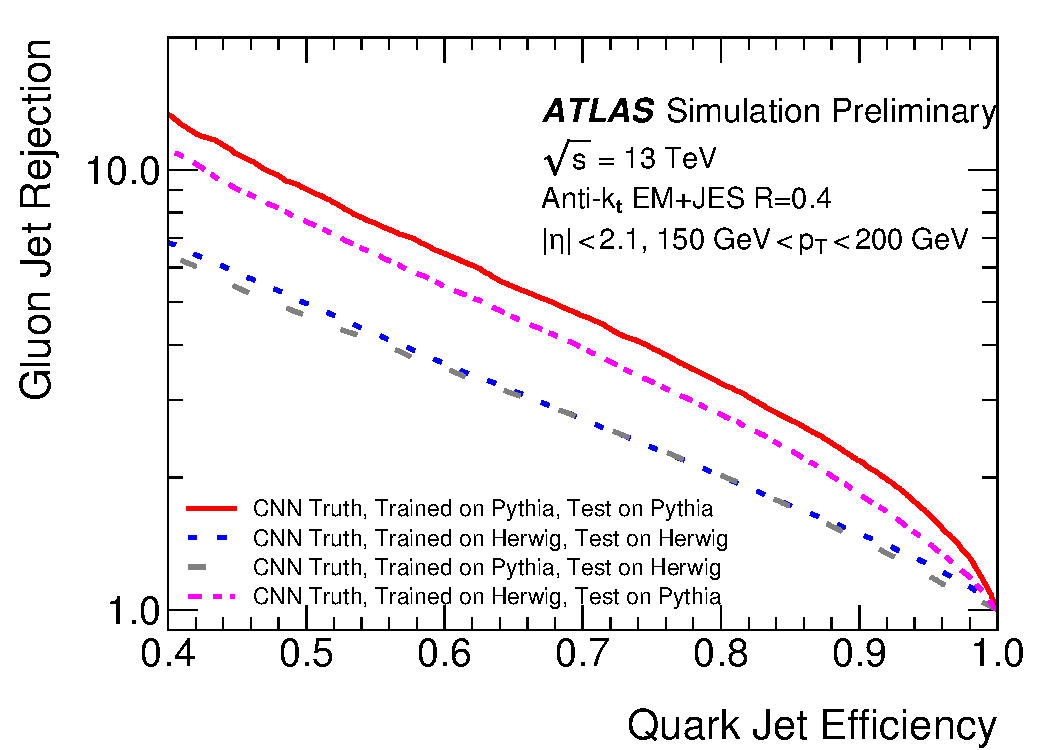
\includegraphics[width=0.5\textwidth]{figures/CNN/ROC_pt150_200_gen_pythia_herwig.pdf}\label{pythiaherwig}} 
\caption{Gluon jet rejection as a function of the quark jet efficiency comparing \textsc{Pythia} to \protect\subref{CNN} \textsc{Sherpa}
and \protect\subref{pythiaherwig} \textsc{Herwig} for jets with $150<\pt<200~\GeV$.}
\label{fig:cnn-pythiasherpa}
\end{center}
\end{figure}



